\chapter{Introduction}
The problem of the transport of a solute arises in many areas of science. In
physiology, examples include the transport of nutrients from the maternal to the
foetal blood in the placenta (see figure~\ref{fig:placenta}; the exchange of oxygen
and carbon dioxide by the alvioli in the lungs (see figure~\ref{fig:alveolus}).

\begin{figure}[ht!]
    \centering
    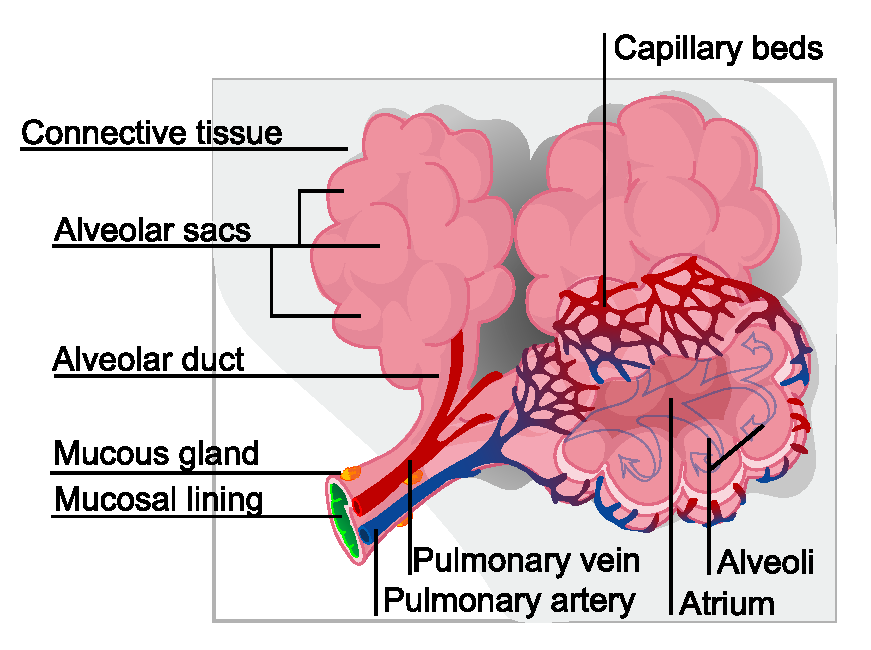
\includegraphics[width=0.7\textwidth]{introduction/figures/alveolus}
    \caption{\label{fig:alveolus}Schematic of an alveolar acini (from
http://en.wikipedia.org/wiki/File:Alveolus\_diagram.svg)}
\end{figure}
\begin{figure}[ht!]
    \centering
    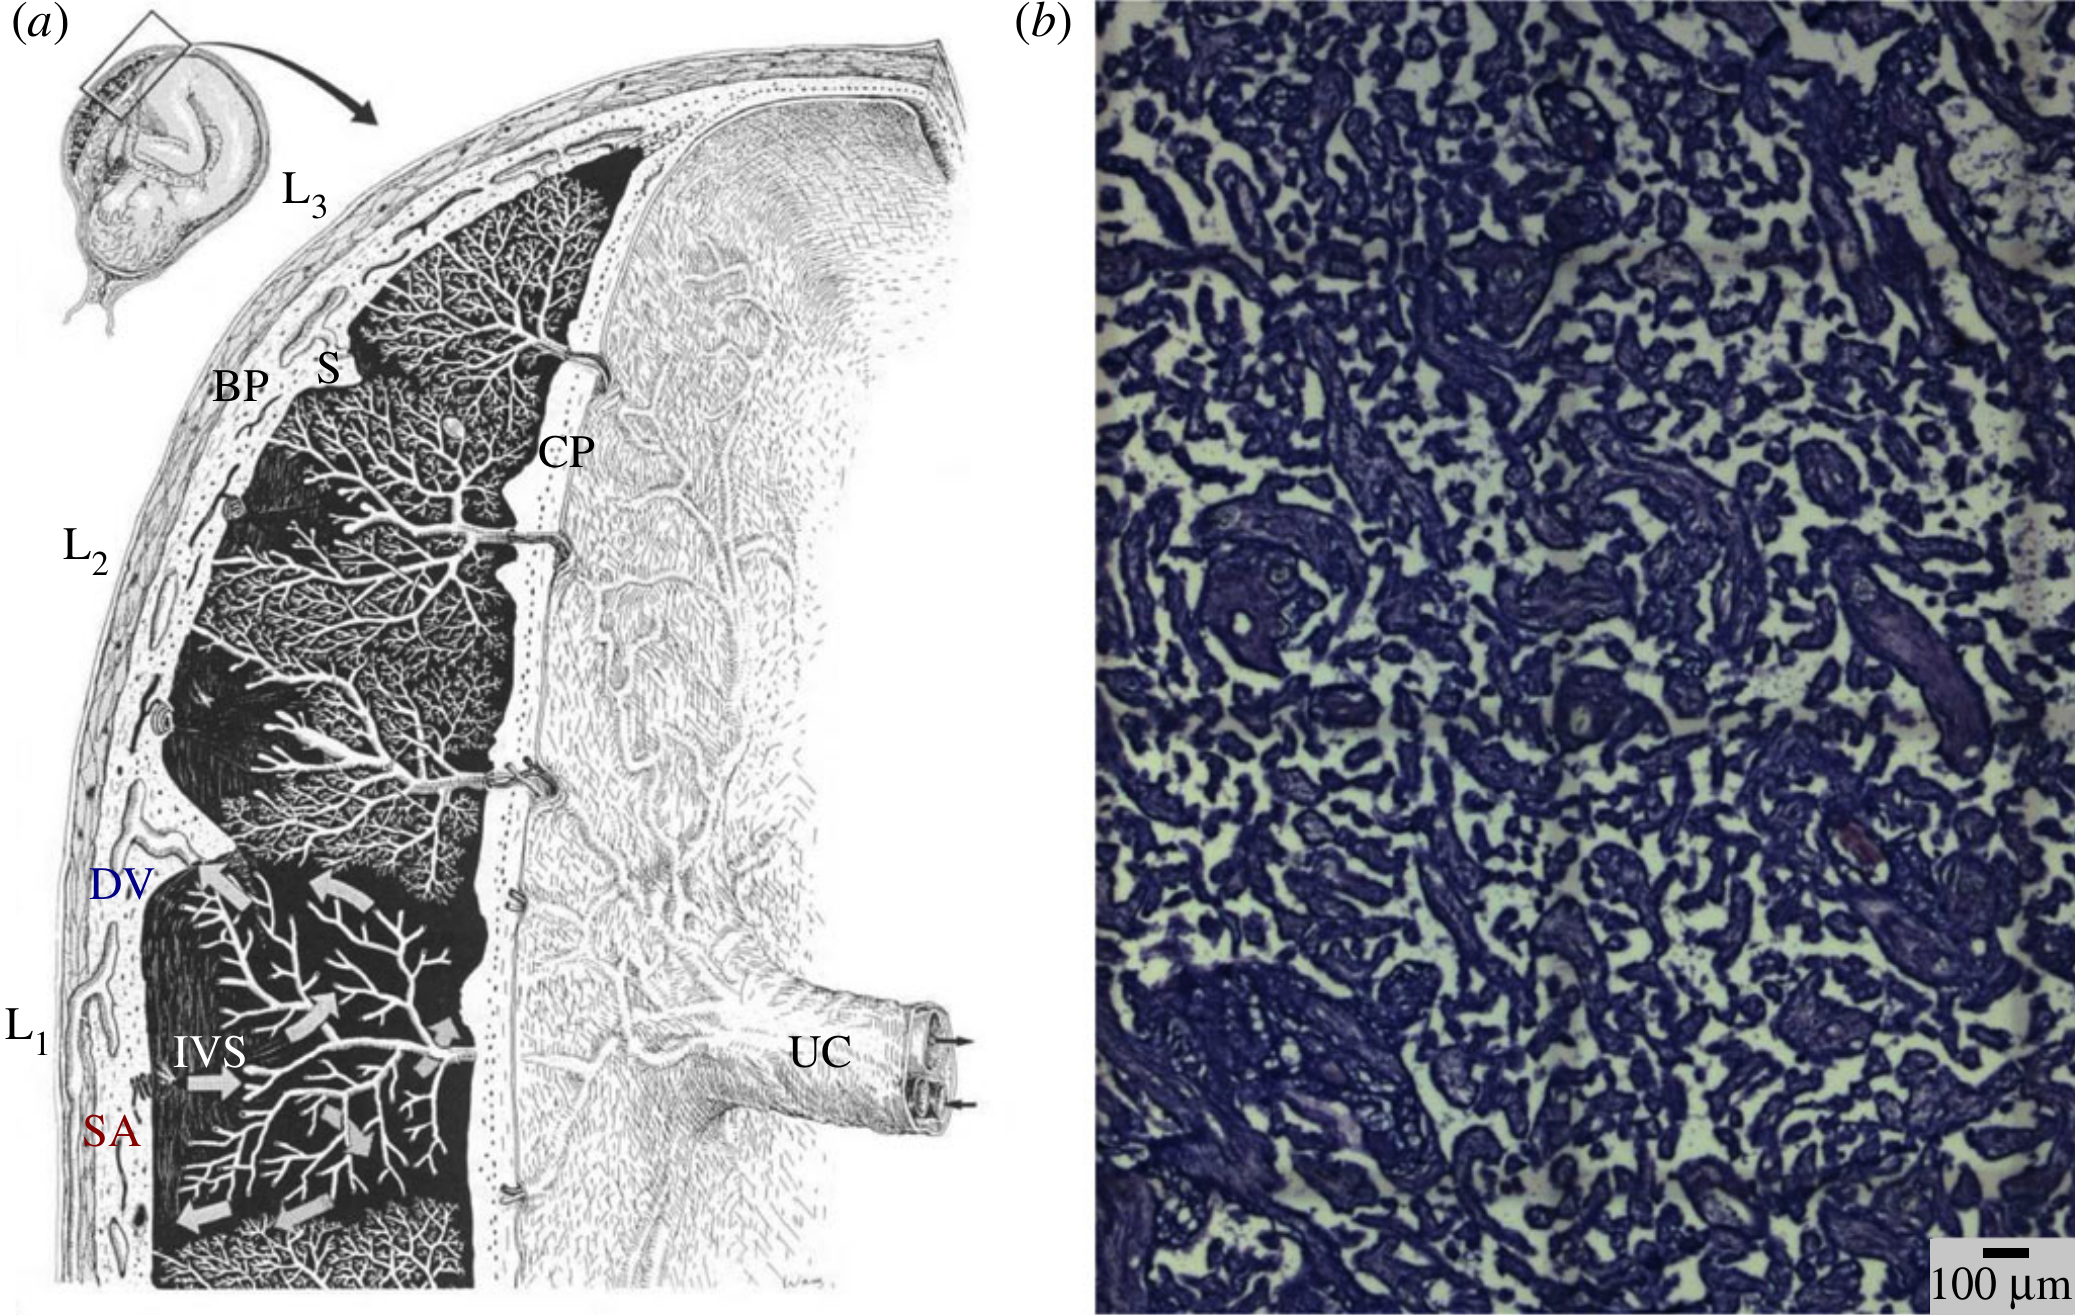
\includegraphics[width=0.7\textwidth]{introduction/figures/placentarast}
    \caption{\label{fig:placenta}Schematic of the placenta (from
    \cite{chernyavsky2012characterizing})}
\end{figure}

\todo{More examples? Other fields - earth science, industry \ldots}

We use two broad approaches to model transport phenomena: continuum models and
agent based models. The relationship between these approaches is another focus
and a goal is to provide a unified model incorporating features of both types of
model.

Both approaches assign a representation of concentration to each
spatial location. In continuum models, physical space is represented as an
interval of the real numbers and the concentration takes positive real values.
In contrast, the most basic individual based models involve finitely many
spatial locations (called ``urns'') and each urn can hold a positive integral
number of particles.

When one begins to take certain limits of the individual based system, the
distinction between the two approaches becomes less well-defined. For example,
one may obtain a continuum model from a discrete model in the appropriate limits
of a large number of urns and large numbers of particles. \todo{clarify, refs}

\section{Literature review}
\todo{write this section\ldots}
\cite{chernyavsky2011transport} \cite{chernyavsky2012characterizing}
others\ldots

\begin{itemize}
    \item Zero range processes (apparently introduced in Interaction of Markov
        Processes (Frank Spitzer))
        \begin{itemize}
            \item There is a mapping from exclusion processes to ZRPs (under
                certain conditions)
            \item ZRPs exhibit a ``condensation transition analogous to
                Bose-Einstein condensation''
            \item It's ``known'' that ZRPs in a 1D periodic domain have a
                factorisable pdf in steady state (Schadscheider et al)
            \item Their exact steady state solution is also ``known''
                (Schadscheider et al)
            \item ``Zero-range process with open boundaries'' gives the
                open-boundaries stationary distribution (our problem)
        \end{itemize}
\end{itemize}

